\documentclass[twocolumn]{article}

% Imports the catppuccin theme, using the mocha flavor,
% from the directory above. Actual implementation
% wouldn't need the import package unless the theme
% and the document are in different directories.
\usepackage{import}
\usepackage{xcolor}
\usepackage{cancel}
\usepackage{mathtools}

% For permutations and combinations
\newcommand\Myperm[2][^n]{\prescript{#1\mkern-2.5mu}{}P_{#2}}
\newcommand\Mycomb[2]{\prescript{#1\mkern-0.5mu}{}C_{#2}}

% Colors
\definecolor{yorhabg}{HTML}{131314}
\definecolor{yorhafg}{HTML}{C9C7CD}
\definecolor{yorhagrid}{HTML}{B5AF9C}
\definecolor{mred}{HTML}{D67069}
\definecolor{mblue}{HTML}{6887A1}

\pagecolor{yorhabg}
\color{yorhafg}

\import{Singularity}{preamble.sty}

% Removes padding above title
\usepackage{titling}
\setlength{\droptitle}{-10em}

% Font package
\usepackage[T1]{fontenc}

\usepackage{fouriernc}

\usepackage{sectsty}
\usepackage{graphicx}
\usepackage{amsmath}
\usepackage{amsfonts}
\usepackage{amssymb}
\usepackage[skins, most]{tcolorbox}

\DeclareMathOperator{\sgn}{sgn}

\usepackage{tikz}
\usepackage{eso-pic}
\usetikzlibrary{calc,shadows.blur}
\usetikzlibrary{angles, quotes}
\usetikzlibrary{3d}

% Margins
\topmargin=0in
\evensidemargin=0in
\oddsidemargin=0in
\textwidth=6.5in
\textheight=9.0in
\headsep=0.25in

\AtBeginEnvironment{tcolorbox}{\small}

\newtcolorbox{imp}{enhanced,arc=0mm,colback=yorhabg,colframe=mred,leftrule=10mm,coltext=yorhafg,%
overlay={\node[anchor=west,outer sep=2pt] at (frame.west) {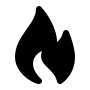
\includegraphics[width=6mm]{images/imageb.png}}; }}

\newtcolorbox{shortcut}{enhanced,arc=0mm,colback=yorhabg,colframe=mred,leftrule=10mm,coltext=yorhafg, coltitle=yorhabg, title=\texttt{Shortcut.}, 
overlay={\node[anchor=west,outer sep=2pt] at (frame.west) {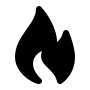
\includegraphics[width=6mm]{images/imageb.png}}; }}

\newtcolorbox{question}{
    enhanced, 
    colback=yorhabg,
    colframe=mblue,
    coltext=yorhafg,
    coltitle=yorhabg,
    attach boxed title to top left={yshift*=-\tcboxedtitleheight}, 
    title=\texttt{Question.},
    boxed title size=title,
    boxed title style={%
        rounded corners=northeast, 
        rounded corners=northwest, 
        colback=tcbcolframe, 
        boxrule=0pt,
    },
    underlay boxed title={%
        \path[fill=tcbcolframe] (title.south west)--(title.south east) 
            to[out=0, in=180] ([xshift=5mm]title.east)--
            (title.center-|frame.east)
            [rounded corners=5pt] |- 
            (frame.north) -| cycle; 
    },
}

\newcommand\bb[1]{\textcolor{yorhafg}{\textbf{#1}}}

\title{\textbf{Subtle Concepts.}}
\author{ Bhuv }
\date{\today}

\begin{document}

\maketitle    

\section*{Change in Potential Energy.}

Change in P.E between any two points is defined as the negative of the work done by the conservative force between those two points.

\[
    U (r_2) - U (r_1) = - \int _{r_1} ^{r_2} \vec{F} \cdot d\vec{r} = - W_{\text{conservative}}
\]

Potential Energy can only be defined at a point with respect to another point. It is not an absolute quantity. It is always defined with respect to a reference point.

\vspace{0.1in}

\begin{imp}
    The statement ``The potential energy of a body at a height $h$ is $mgh$'' is incorrect. The correct statement would be ``The potential energy of a body at a height $h$ with respect to the ground is $mgh$''. 
\end{imp}

\vspace{0.1in}

In most cases to get a unique value, we take the reference point as \(\infty\), where the potential energy is zero. 

\[
    U (r) = - \int_{\infty} ^{r} \vec{F} \cdot d\vec{r} = - W
\]

\vspace{0.1in}

\begin{question}
    A conservative force field function is given by \(F = \dfrac{k}{r^{2} }\), where \(k\) is a constant.
    \vspace{0.1in}

    (a) Determine the potential energy function \(U(r)\) assuming zero potential energy at \(r = r_0\).

    \vspace{0.1in}
    (b) Also, determine the potential energy at \(r = \infty\). 
\end{question}

(a) Since potential energy is 0 at \(r = r_0\), we consider \(r_0\) as the reference point. 

\[
    U(r) - U(r_0) = -\int_{r_0} ^{r} F dr =  - \int_{r_0} ^{r} \dfrac{k}{r^{2} } dr
\]

We know that \(U (r_0) = 0\). 

\[
    U(r) = [\frac{k}{r}]_{r_0} ^{r} 
\]

\[
    \boxed{U(r) = k (\frac{1}{r} - \frac{1}{r_0})}
\]

(b) For \(\infty\), 

\[
    U(\infty) = - \int_{r_0} ^{\infty} \frac{k}{r^{2} } dr 
\]

\[
    U(\infty) = [\frac{k}{r}]_{r_0} ^{\infty}
\]

\[
    \boxed{U(\infty) = - \frac{k}{r_0}}
\]

\vspace{0.1in}
\hrule

\begin{question}
    This system is released from rest. Find the relation between the velocity of the COM and the angular velocity (about \(C\)).
    \begin{center}
        \begin{tikzpicture}[scale=1]
            % Define parameters
            \def\L{4}        % Length of the rod
            \def\t{30}   % Angle in degrees
            
            % Draw the ground (horizontal line)
            \draw[line width=3pt] (-1,0) -- (5,0);
            
            % Define endpoints A and B of the rod
            \coordinate (A) at (0,0);
            \coordinate (B) at ({\L*cos(\t)},{\L*sin(\t)});
            
            % Draw the rod
            \draw[line width=2pt, mblue] (A) -- (B);
            
            % Label endpoints A and B
            \node[below left] at (A) {$A$};
            \node[above right] at (B) {$B$};
            
            % Mark and label the midpoint C of the rod
            \coordinate (C) at ($(A)!0.5!(B)$);
            \filldraw[mred] (C) circle (3pt);
            \node[above left] at (C) {$C$};
            \draw[->] (C) -- (1.7, 0.5) node[right] {\(v_c\) };
            
            % Draw an arc to indicate the angle theta at A
            \draw (0.5,0) arc (0:\t:0.5);
            \node at ({0.5*cos(\t/2) + 0.3}, {0.8*sin(\t/2)}) {$\theta$};
          \end{tikzpicture}
    \end{center}
\end{question}

The velocity of the point A normal to the ground is 0. So, at point A

\[
    \frac{\omega l}{2} \cos \theta - v_c = 0
\]

Therefore, 
\[
    \boxed{\omega = \frac{2v_c}{l \cos \theta }}
\]

\vspace{0.1in}
\hrule

\begin{question}
    Find the M.I of the system consisting of solid spheres and a rod connecting them about the axis. \(a\) is the distance from the C.O.M of rod. 
    \begin{center}
        \begin{tikzpicture}[scale=1]

            \draw (0, 0) circle (0.5) node{\(m_1, r_1\) } ;
            \draw (5, 0) circle (0.8) node{\(m_2, r_2\) };

            \draw[thick] (0.5, 0) -- (5-0.8, 0) node[midway, below right]{\(l, m\)};

            \draw[dashed, mred, thick] (1.25, -1) -- (1.25, 1) node[right]{Axis};
            \draw[<->] (1.25, 0.5) -- (2.5, 0.5) node[right]{\(a\) }; 

          \end{tikzpicture}
    \end{center}
\end{question}

The total M.I is the sum of individial M.I of the masses around the axis. So, 

\[
    I_{\text{axis} } = I_{1,a} + I_{2,a} + I_{m,a} 
\]

M.I of sphere 1 about the axis will be, 
\[
    I_{1,a} = \frac{2}{5}m_1 r_{1}^{2} + m_1 (r_1 + \frac{l}{2} - a)^{2} 
\]

Similarly, 
\[
    I_{2,a} = \frac{2}{5}m_2 r_{2}^{2} + m_2 (r_2 + \frac{l}{2} + a)^{2}
\]

\[
    I_{m,a} = \frac{ml^{2}}{12} + ma^{2} 
\]

And so, the total M.I of the system will be the sum of these three. 

\vspace{0.1in}
\hrule 

\begin{question}
    If the system is at equilibrium, find 
    \begin{itemize}
        \item[(i)] Normal reaction by ground on ladder. 
        \item[(ii)] Normal reaction by wall on ladder. 
        \item[(iii)] Frictional force on the ladder. 
        \item[(iv)] Net force exerted by ground on ladder.    
    \end{itemize}
    \begin{center}
        \begin{tikzpicture}[scale=1]

            \draw[line width=1.5pt] (0, 5) -- (0, 0) coordinate (o) -- (5, 0);
            \draw[thick, mblue] (3, 0) coordinate (x) -- (0, 4) coordinate (y) node[midway, right]{\(M,\ L\) };
            \pic [draw, <->,
                angle radius=9mm, angle eccentricity=1.2,
                "$\theta$"] {angle = y--x--o};

            \draw[->, mred] (0, 4) -- (1, 4) node[right]{ \(N_w\) };
            \draw[->, mred] (3, 0) -- (3, 1) node[right]{ \(N_g\)  };

          \end{tikzpicture}
    \end{center}
\end{question}

Alright, so equating the vertical forces, we get 

\[
    N_g = Mg
\]

Equating the Horizontal forces, 

\[
    N_w = f
\]

Now, balancing the torque about the C.O.M 

\[
    N_w (\frac{L}{2}) \sin \theta = N_g (\frac{L}{2}) \cos \theta - f(\frac{L}{2}) \sin \theta  
\]

\[
    (N_w + f) \sin \theta = N_g \cos \theta 
\]

\[
    \boxed{f = \frac{Mg \cot \theta }{2}}
\]

And the net force on the ladder by the ground will be, 

\[
    F_n = \sqrt{(N_g)^{2} + (f)^{2} } 
\]

\[
    \boxed{F_n = \frac{Mg}{2}\sqrt{4 + \cot ^{2} \theta } }
\]

\vspace{0.1in}
\hrule

\begin{question}
    Find the maximum mass \(M\) that can be suspended before the beam slips. Also, determine the magnitude of the reaction force at the floor and magnitude of force exerted by the beam on the rope at \(P\) in terms of \(m, M, \mu_s\). 
    \begin{center}
        \begin{tikzpicture}
            \draw (0, 0) coordinate (o) -- (4, 0) node[midway, below left]{\(\mu \) };
            \draw[line width=4pt, opacity=0.4] (4, 0) -- (4, 4);
            \draw (4, 3) -- (1, 3) coordinate (y);
            \draw[thick, mblue] (1, 3) -- (3, 0) coordinate (x) node[midway, right]{\(m\) };
            \draw (1, 3) -- (1, 1.5) node[below, draw, mred] {\(M\) };
            \pic [draw, <->,
                angle radius=7mm, angle eccentricity=1.2,
                "$\theta$"] {angle = y--x--o};
        \end{tikzpicture}
    \end{center}
\end{question}

For equilibrium of a rigid body, the vertical and horizontal forces should be in equilibrium and the net torque on the system should be 0. 

\begin{center}
    \begin{tikzpicture}
        \draw (0, 0) coordinate (o) -- (4, 0);
        \draw[thick, mblue] (1, 3)  coordinate (y) -- (3, 0) coordinate (x);
        \draw[->, mred] (1, 3) -- (1, 2) node[left]{\(Mg\) };
        \draw[->] (1, 3) -- (2, 3) node[right]{\(T\) };
        \draw[->] (3, 0) -- (3, 1) node[right]{\(N\) };
        \draw[->] (3, 0) -- (2, 0) node[below]{\(\mu N\) };
        \draw[->, mblue] (2, 1.5) -- (2, 0.5) node[left]{\(mg\) };
        
    \end{tikzpicture}
\end{center}

Along the vertical direction, 
\[
    N = (m + M)g
\]

Horizontally,
\[
    \mu N = T
\]

Balancing the torque around the C.O.M of the rod, 

\[
    T \sin \theta + \mu N \sin \theta = N \cos \theta + Mg \cos \theta
\]

\[
    2 \mu N \sin \theta = (m + 2M)g\cos \theta 
\]

\[
    2 mg \mu \sin \theta + 2Mg \mu \sin \theta = mg \cos \theta + 2Mg \cos \theta 
\]

\[
    m(2\mu \sin \theta - \cos \theta) = 2M (\cos \theta - \mu \sin \theta )
\]

Therefore, 

\[
    \boxed{M_{\text{max} } = \frac{m}{2} (\frac{2\mu \sin \theta - \cos \theta }{\cos \theta - \mu \sin \theta})}
\]

Now, the magnitude of reaction force at the floor will be,

\[
    F_{\text{floor} }  = \sqrt{N^{2} + (\mu N)^{2} }
\]

\[
    \boxed{F_{\text{floor} } = (m + M)g \sqrt{1 + \mu ^{2} }}
\]

And now, the force on the rope by the beam will be,

\[
    F_{\text{rope, beam} } = \sqrt{T^{2} + (Mg)^{2} }  
\]

\[
    \boxed{F_{\text{rope, beam} } = \sqrt{\mu ^{2} (m + M)^{2} g^{2} + M^{2} g^{2} }  }
\]

\vspace{0.1in}
\hrule 

\begin{question}
    Find the acceleration of \(m_1\) and \(m_2\) if there is friction between the rope and pulley. 
    \begin{center}
        \begin{tikzpicture}
            \draw (0, 0) circle (1) node[right]{\(I\) };
            \draw (-2, 1.5) -- (2, 1.5);
            \draw[thick] (0, 1.5) -- (0 ,0);
            \draw (-1, 0) -- (-1, -2) node[below, draw, mred]{\(m_2\) };
            \draw (1, 0) -- (1, -2) node[below, draw, mblue]{\(m_1\) };
            \draw[->] (-1.5, -1.5) -- (-1.5, -0.5) node[midway, left]{\(a\) };
            \draw[->] (1.5, -0.5) -- (1.5, -1.5) node[midway, right]{\(a\) };
        \end{tikzpicture}
    \end{center}
\end{question}

Now here, we don't take Tension to be equal at all points on the rope as there is force applied by the pulley on the rope due to friction. So, for \(m_2\),

\[
    T_2 = m_2 (g + a)
\]

for \(m_1\),
\[
    T_1 = m_1 (g - a)
\]

Now, the torque on the pulley will be the difference between the tension. 

\[
    \tau = (T_1 - T_2)R = I \alpha 
\]

\[
    \alpha = \frac{a}{R} = \frac{(T_1 - T_2)R}{I}
\]

\[
    a = (T_1 - T_2) \frac{R^{2}}{I}
\]

Now, 

\[
    T_1 - T_2 = m_1 (g - a) - m_2 (g + a)
\]

\[
    a \frac{I}{R^{2} } = (m_{1} - m_2)g - (m_1 + m_2)a 
\]

Therefore, 

\[
    \boxed{a = \frac{(m_{1} - m_2)g}{m_1 + m_2 + \frac{I}{R^{2} }}}
\]

\vspace{0.1in}

\begin{shortcut}
    Before, without friction between rope and pulley we had, 
   \[
       a = \frac{(m_{1} - m_2)g}{m_1 + m_2}
   \]
   After friction in pulley, 
   \[
       a = \frac{(m_{1} - m_2)g}{m_1 + m_2 + \frac{I}{R^{2} }}
   \]

   This result can also be applied to a few other cases to save time. 

\end{shortcut}

\vspace{0.1in}
\hrule

\begin{question}
    The radius of both is the same \(R\). As \(M_2\) rolls down, the string gets unwound. Find the acceleration of \(M_2\).
    \begin{center}
        \begin{tikzpicture}
            \draw (0, 0) circle (1) node[right]{\(M_1\) };
            \draw (-2, 1.5) -- (2, 1.5);
            \draw[thick] (0, 1.5) -- (0 ,0);
            \draw (1, 0) -- (1, -3);
            \draw (2, -3) circle (1) node{\(M_2\) };
            \draw[->] (1.5, -0.5) -- (1.5, -1.5) node[midway, right]{\(a\) };
        \end{tikzpicture}
    \end{center}
\end{question}

Drawing the FBD of shit. 

\begin{center}
    \begin{tikzpicture}
        \draw (0, 0) circle (1) node[right]{\(M_1\) };
        \draw (-2, 1.5) -- (2, 1.5);
        \draw[thick] (0, 1.5) -- (0 ,0);
        \draw[->, mred] (1, 0) -- (1, -1) node[right]{\(T\) };
        \draw[->, mred] (1, -3) -- (1, -2) node[left]{\(T\) };
        \draw[->, mblue] (2, -4) -- (2, -5) node[right]{\(M_2 g\) };
        \draw[->, mblue] (2, -2) -- (2, -1) node[right]{\(M_2 a\) };

        \draw[fill] (1, 0) circle (0.05) node[right]{\(P\) };
        \draw[fill] (1, -3) circle (0.05) node[left]{\(Q\) };

        \draw (2, -3) circle (1) node{\(M_2\) };
    \end{tikzpicture}
\end{center}

Analysing \(M_2\),

\[
    T = M_2 (g - a) \tag{1}
\]

Analysing the torque of \(M_2\), 

\[
    TR = \frac{M_2 R^{2}}{2} \alpha_2 
\]

\[
    \alpha_2 = \frac{2T}{M_2 R} \tag{2}
\]

Similarly, 
\[
    \alpha_1 = \frac{2T}{M_1 R} \tag{3}
\]

Now comes the constraint equation. We can see that P and Q are from the same string, so they must have equal acceleration. Therefore, 

\[
    a_{Q} = \alpha_2 R - a 
\]

\[
    a_{P} = \alpha_1 R 
\]

Equating them, 

\[
    a = (\alpha_2 - \alpha_1) R \tag{4}
\]

Now substituting (1) in (2) and (3) and then substituting the values of \(\alpha_1\) and \(\alpha_2\) in (4), we get, 

\[
    \boxed{a = [\frac{2(M_1 + M_2)}{3M_1 + 2M_2}]g}
\]

\vspace{0.1in}
\hrule

\begin{question}
    A uniform cylinder of mass \(M\) and radius \(R\) is kept on an accelerating platform (mass \(M\) ) as shown. If the cylinder rolls without slipping on the platform, determine the magnitude acceleration of the C.O.M of the cylinder. Assuming the coefficient of friction \(\mu\), determine the maximum acceleration the platform my have without slip between cylinder and the platform. 
    \begin{center}
        \begin{tikzpicture}
            \draw (0, 0) circle (1) node[right]{\(M\) };
            \draw[line width=5pt] (1.5, -1.1) -- (-1.5, -1.1) node[left]{\(M\) };
            \draw[->] (1.5, -1.1) -- (2, -1.1) node[right]{\(a\) };
        \end{tikzpicture}
    \end{center}
\end{question}

Now here, the thing that is causing the rotation and movement of the cylinder is the friction between the cylinder and the platform. So,

\[
    a_c = \frac{f}{M}
\]

Moreover, the rotation too is caused only by the friction force, so 

\[
    \alpha = \frac{2f}{M R}
\]

And also, analysing the point of contact, the total acceleration of that point should be equal to the acceleration of the platform. 

\[
    a = a_c + \alpha R
\]

\[
    f = \frac{Ma}{3}
\]

And since there's no slipping, 

\[
    f \leq  \mu Mg
\]

\[
    \frac{Ma}{3} \leq  \mu Mg
\]

Therefore, 

\[
    \boxed{a_{\text{max}} = 3\mu g}
\]

\vspace{0.1in}
\hrule

\section*{Electrostatic Pressure.}

We find the pressure that exists on charged bodies. This is the stress that motivates charged bodies to just rip off and fly apart but is held by mechanical forces (tension) of the conductor. 

So first, lets take a small elemental part \(dq\). Now, The force experienced by this shit will be,

\[
    dF = dq(E_2)
\]

Now, \(E_2\) is the electric field due to the rest of the body except \(dq\) and \(E_1\) is the field due to \(dq\). Taking a point inside the conductor, we know that the net electric field is 0. 

\[
    E_1 - E_2 = 0 \implies E_1 = E_2
\]

We also know from Gauss' Law that the field just outside the surface of the conductor will be 

\[
    E_1 + E_2 = \frac{\sigma}{\epsilon_0}
\]

\[
    E_2 = \frac{\sigma}{2\epsilon_0}
\]

Substituting, 

\[
    dF = (\frac{\sigma}{2\epsilon_0}) dq
\]

We know that, \(dq = \sigma dA\)

\[
    dF = (\frac{\sigma^{2}}{2 \epsilon_0})dA 
\]

\[
    \frac{dF}{dA} = \frac{\sigma^{2}}{2\epsilon_0}
\]

Now, since the net external field outside the conductor is \(E_{\text{external}} = \dfrac{\sigma}{\epsilon_0} \),

\[
    \boxed{\frac{dF}{dA} = P = \frac{\epsilon_0 E_{\text{ext} }^{2}}{2} }
\]

\vspace{0.1in}
\hrule 

\end{document}

